\subsection{Empirical Findings}
\label{sec:empirical}

We apply $\ell_z^*$ to 12 models across five benchmarks (60 model-benchmark cells).
After Benjamini--Hochberg FDR correction ($\alpha=0.05$), 57 of 60 cells are flagged as significant.
The three unflagged cells (Yi-Lightning$\times$ARC-C, 360GPT2-Pro$\times$HumanEval, Yi-Lightning$\times$HumanEval) all involve small benchmarks ($n \leq 295$), consistent with the power analysis in \S\ref{sec:simulation}.
By contrast, a simple accuracy $z$-score baseline (standardized accuracy across models per benchmark) flags only 4 of 60 cells: $\ell_z^*$ captures 14$\times$ more anomalies by exploiting response-pattern structure that accuracy aggregation discards.
This near-universal misfit indicates that real LLM response patterns systematically deviate from 4PL IRT predictions, regardless of architecture or training paradigm.

\paragraph{12-model case study.}
Figure~\ref{fig:heatmap} presents the $\ell_z^*$ heatmap across 12 models and five benchmarks.
93.0\% of flagged cells exhibit positive $\ell_z^*$ (over-consistency): models answer too many hard items correctly relative to their estimated ability.
Gemini-1.5 on MMLU represents an extreme case: near-perfect accuracy, $\hat{\theta}=0.78$, and $\ell_z^*{=}{+}31.81$, with 50 of 57 MMLU subjects flagged individually.
Ward hierarchical clustering on the $\ell_z^*$ profile matrix reveals heterogeneous contamination typologies; Gemini-1.5 isolates as a distinct outlier, while other models form clusters that correspond to selective versus uniform misfit.
Ten of 12 models are flagged on all five benchmarks simultaneously.

\paragraph{IRT parameter estimation gap.}
A 3PL refit via MML-EM on the v1 leaderboard ($N{=}178$ models) recovers difficulty moderately ($r_b = 0.663$) but fails on discrimination ($r_a = 0.127$).
Classical IRT calibration requires sample sizes that current leaderboards cannot provide; neural calibration methods such as PSN-IRT \citep{psnirt2026} remain essential.
On real data, 4PL and 3PL $\ell_z^*$ values correlate at only $r=0.225$ (RMSE$\,{=}\,68.41$), which confirms that the guessing-slip parameters ($c$, $d$) captured by 4PL substantially alter person-fit assessment.
This simulation-to-reality gap constitutes an informative negative result: it quantifies the boundary conditions under which classical IRT calibration degrades.

\begin{figure}[t]
  \centering
  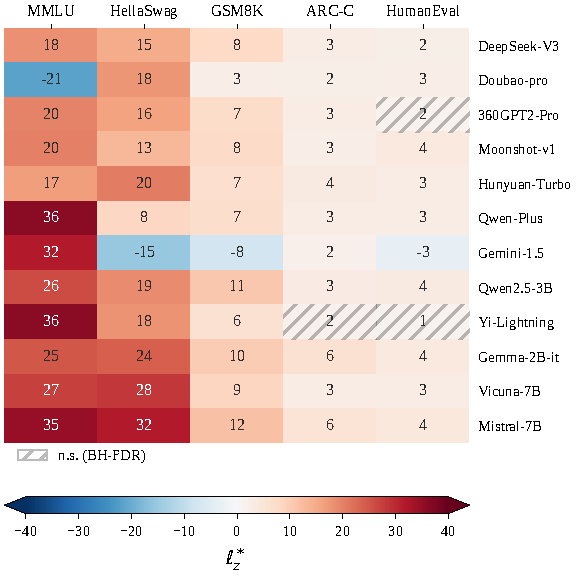
\includegraphics[width=\columnwidth]{fig_4_model_heatmap.pdf}
  \caption{$\ell_z^*$ heatmap for 12 models across five benchmarks. Positive values (red) indicate over-consistent response patterns. Gemini-1.5 on MMLU ($\ell_z^*{=}{+}31.81$) is an extreme outlier. Ward clustering (left dendrogram) reveals distinct contamination typologies.}
  \label{fig:heatmap}
\end{figure}
